% XeLaTeX
% 使用minted宏包 
% 运行的时候需要加一个参数即:-shell-escape
% 使用minted宏包新定义了cppcode环境,可直接使用
\documentclass{article}
\usepackage{geometry}
\usepackage{ctex}
\usepackage{minted}
\usepackage{hyperref}


\newminted{matlab}{mathescape,
               linenos,
               numbersep=5pt,
               gobble=2,
               frame=lines,
               framesep=2mm,
               breaklines=true}
\geometry{left=2cm,right=2cm,top=2.5cm,bottom=2.5cm}
\def\figureautorefname{图}%
\hypersetup{hidelinks}

\begin{document}

\title{homework 10.13}
% \subtitle{in course of probability theory}
\author {王永锋 16337237 教务三班}
\maketitle
% \tableofcontents

\section{题目}
请用matlab 编程语言实现求解下列问题,设随机变量 \( X~N(2, 0.25) \)

\begin{itemize}

\item 求概率P\{0.5<X<2.5\};
\item 绘制分布函数图和分布密度图;
\item 画出区间[1.5, 1.9] 上的分布密度曲线下方区域。

\end{itemize}

\subsection{第一题}
由题目可知,随机变量 \( X \) 符合参数为2,0.25的正态分布 \

直接用内置函数normspec即可解决

\begin{matlabcode}
    normspec([0.5,2.5],2,0.5)
\end{matlabcode}
得出概率为
\[ P\{0.5<X<2.5\} \approx 0.84 \]

\clearpage

结果如\autoref{img:1}所示
\begin{figure}[!thbp]
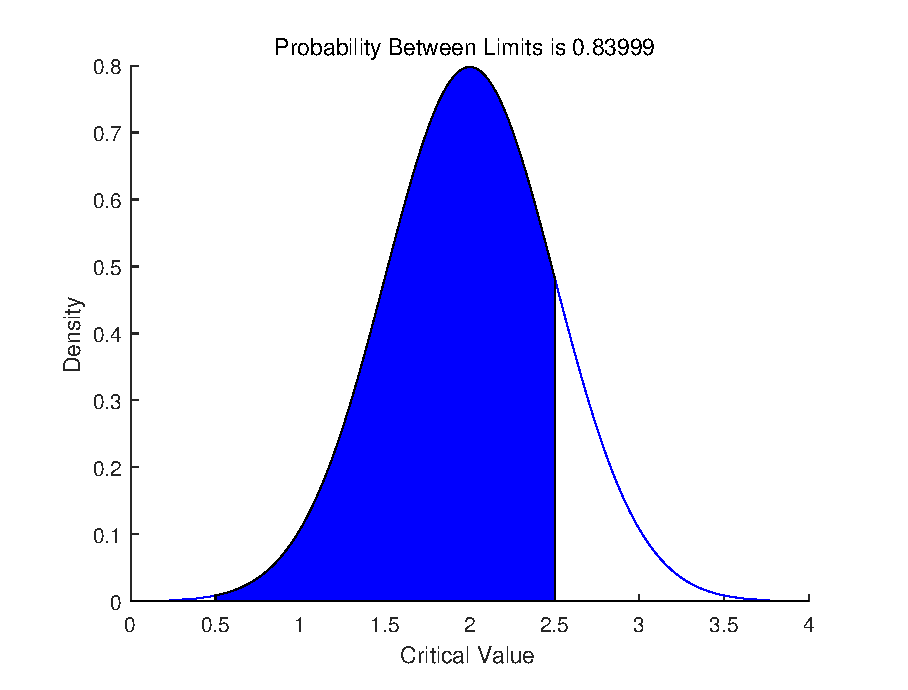
\includegraphics[width=.5\textwidth]{1.eps}
\centering
\caption{参数为2,0.25的正态分布,随机变量落在0.5到2.5之间的概率} 
\label{img:1}
\end{figure}


\subsection{第二题}
求解第二题所使用的代码
\begin{matlabcode}

    clc
    clear
    % 概率密度函数图
    figure
    x = 0:0.01:4;
    y1 = normpdf(x, 2, 0.5);
    plot(x, y1, 'r');
    title('数学期望为2,方差为0.25的正态分布的概率密度函数图');
    xlabel('随机变量X的取值');
    ylabel('概率密度');

    % 分布函数图
    figure
    y2 = normcdf(x, 2, 0.5);
    plot(x, y2)
    title('数学期望为2,方差为0.25的正态分布的分布概率函数图');
    xlabel('随机变量X的取值');
    ylabel('P{X <= x}');

\end{matlabcode}

结果如\autoref{img:2}, \autoref{img:3}所示

\begin{figure}

\begin{minipage}[t]{0.5\textwidth}%并排放两张图片,每张占页面的0.5,下同。  
\centering  

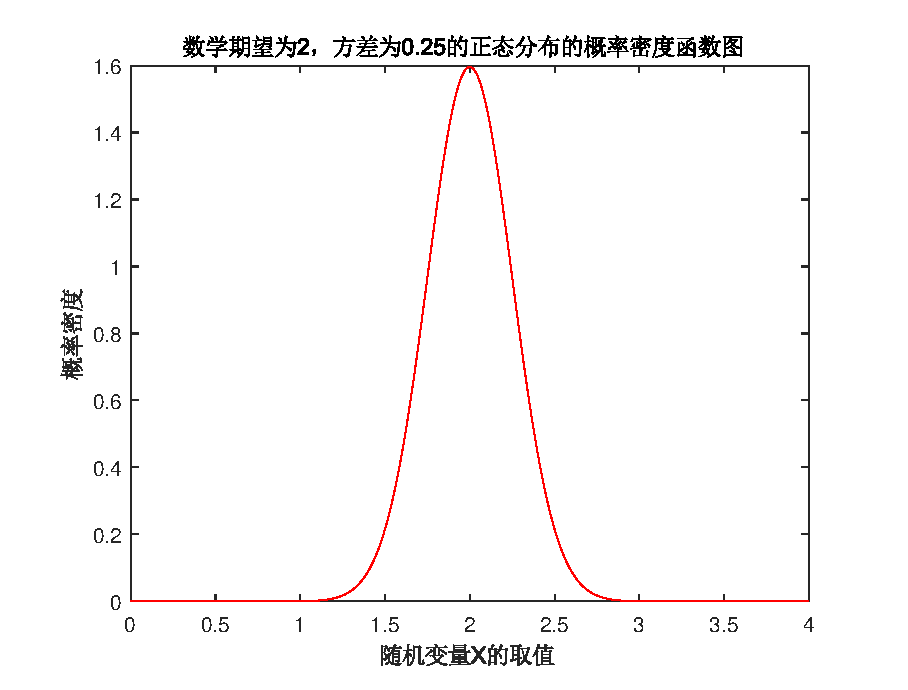
\includegraphics[width=\textwidth]{2.eps}  

\caption{参数为2,0.25的正态分布的分布函数图像} \label{img:2} 
\end{minipage} 
\begin{minipage}[t]{0.5\textwidth}  
\centering  
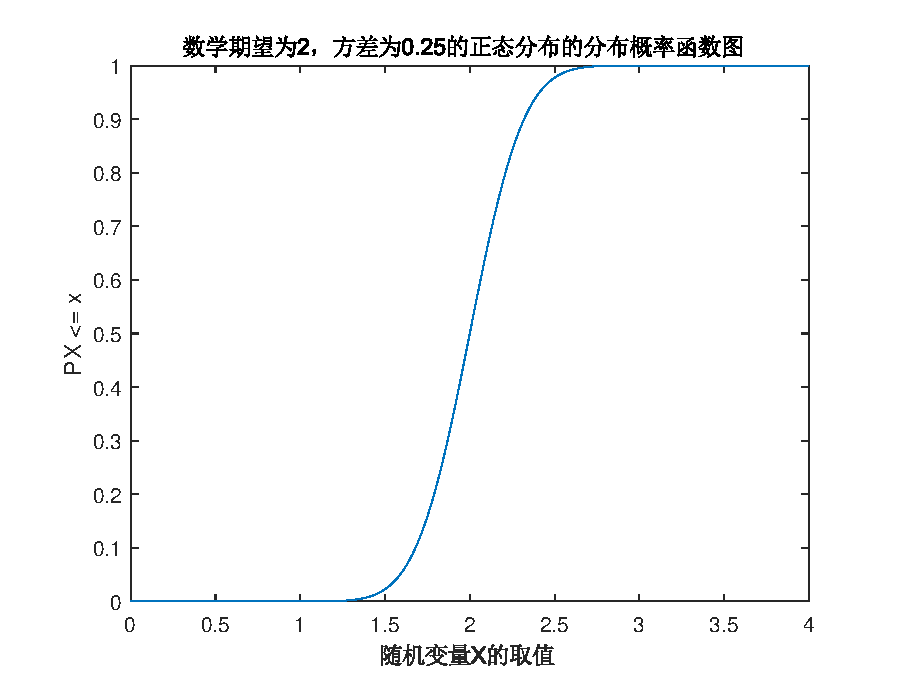
\includegraphics[width=\textwidth]{3.eps}   
\caption{概率密度函数图像.jpg}   \label{img:3} 
\end{minipage}  

\end{figure}  

\subsection{第三题}
题目求解代码如下所示
\begin{matlabcode}

    % 第三题
    % 画出区间[1.5, 1.9] 上的分布密度曲线下方区域。

    figure
    x = 1:0.01:3;
    x3 = 1.5:0.01:1.9;
    y = normpdf(x, 2, 0.5);
    y3 = normpdf(x3, 2, 0.5);
    plot(x, y) % 先画出原有的图像
    hold on % 切换状态
    area(x3, y3) % 在原有的图像上叠加
    title('区间[1.5, 1.9] 上的概率密度曲线下方区域');
    xlabel('随机变量X');

\end{matlabcode}

结果如\autoref{img:4}所示
\begin{figure}[t]
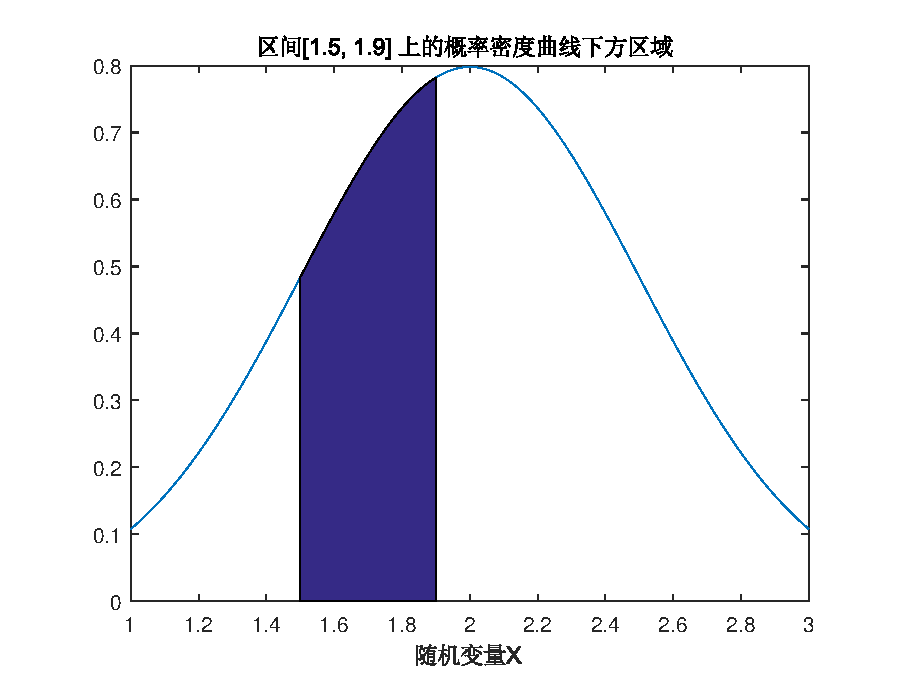
\includegraphics[width=.5\textwidth]{4.eps}
\centering
\caption{参数为2,0.25的正态分布,随机变量在1.5-1.9之间} 
\label{img:4}
\end{figure}


\end{document}